\documentclass{ximera}
\usepackage[UTF8]{ctex}
\usepackage{graphicx}

\title{MA150 Algebra}
\author{于峥}

\begin{document}
\begin{abstract}
    homework 8
\end{abstract}

\maketitle

\begin{problem} Page 88-12
    \begin{solution}
        $U_5$ 是一个5阶循环群,令$U_5 = \langle u \rangle$。

        假设$\phi(x)=u^{x^{'}}$, 则$\phi(x+y)=\phi(x)\phi(y)=u^{x^{'}}\cdot u^{y^{'}}$。

        令$\psi(x)=x^{'}$, 则$\psi(x+y)=\psi(x)+\psi(y)(\mod 5)$,
        
        即$\psi(xy)=x\psi(y)=y\psi(x) \Rightarrow \psi(5x)=0$。

        同时$\psi(y) = y\psi(1) (\mod 5) \Rightarrow \psi(y) = \psi(1)(y \mod 5)$。

        而$\psi(1)$不能为$0$, 否则$\phi$不是满同态。所以
        $\phi(\overline{x}) = 1$ 当且仅当 $\psi(x)=0\Rightarrow x \mod 5 = 0$。

        所以$Ker(\phi) = \{
            \overline{0},    
            \overline{5},    
            \overline{10},    
            \overline{15},    
            \overline{20},    
            \overline{25}\}$。
    \end{solution}
\end{problem}

\begin{problem} Page 89-20
    \begin{solution}
        构造$\mathbb{Z}_m \rightarrow \mathbb{Z}_k : \phi(\overline{{x}})=\overline{x}$。

        $\forall \overline{x} \in \mathbb{Z}_k$, $\exists \overline{x} \in \mathbb{Z}_m$, 所以$\phi$是满同态。

        易发现
        $$
        \begin{aligned}
            Ker \phi &= \{ \overline{x} | \phi(\overline{x}) = \overline{0}\} \\
            &= \{ \overline{x} | x = ak, a \in \mathbb{Z}_+\} \\
            &= \langle \overline{k} \rangle
        \end{aligned}
        $$

        根据群同态定理
        $$
            \mathbb{Z}_m / \langle \overline{k} \rangle \cong \mathbb{Z}_k
        $$
    \end{solution}
\end{problem}

\begin{problem} Page 104-1
    \begin{solution}
        (1)
        $$
        \begin{aligned}
        S_1 &= S_2 =S_3 =S_4 =S_5 = S_6 = \{(1), (78)\} \\ 
        S_7 &= S_8 = \{(1), (123)(456),(132)(465)\} 
        \end{aligned}
        $$
        $$
        \begin{aligned}
            O_1 &= O_2 = O_3 = \{ 1, 2, 3 \} \\
            O_4 &= O_5 = O_6 = \{ 4, 5, 6 \} \\
            O_7 &= O_8 = \{ 7, 8 \}
        \end{aligned}
        $$
        (2)
        $$
        \begin{aligned}
            F_{(1)} &= X \\
            F_{(123)(456)} &= F_{(132)(465)} = \{ 7, 8 \} \\
            F_{(78)} &= \{ 1, 2, 3, 4, 5, 6 \} \\
            F_{(123)(456)(78)} &= F_{(132)(465)(78)} = \emptyset
        \end{aligned}
        $$
    \end{solution}
\end{problem}

\begin{problem} Page 104-3
    \begin{solution}
        由于$G$在$X$上作用是传递的,所以$\forall x, y \in X$, $\exists g \in G, gx = y$。
        考虑 $O_x$,$O_y$,构造映射$O_x \rightarrow O_y : \phi(hx) = ghg^{-1}y$。

        (1) 因为$N$是正规子群,$h \in N$, $ghg^{-1} \in N$,所以显然$\phi$是$O_x$到$O_y$的映射。

        (2) $\forall h_1, h_2 \in N, h_1x = h_2x$,
        $$
        \begin{aligned}
            \phi(h_1x) &= gh_1g^{-1}y \\
            &= gh_1x \\
            &= gh_2x
        \end{aligned}
        $$
        所以$\phi$是单射。

        (3) $\forall h_1, h_2 \in N$,
        $$
        gh_1g^{-1}y = gh_2g^{-1}y \Rightarrow h_1x = h_2x
        $$
        所以$\phi$是满射。

        综上$|O_x|=|O_y|$,由于$x$,$y$的任意性,$X$在$N$作用下的的每个轨道有同样的元素。
    \end{solution}
\end{problem}

\begin{problem} Page 104-4
    \begin{solution}
        $$
            S_x = \{ g \in G| g(x) = x \}
        $$
        (1) $\forall h \in S_x$, 
        $$
        \begin{aligned}
            ghg^{-1}y &= gh(g^{-1}g)x \\
            &=g(hx) \\
            &=gx \\
            &=y
        \end{aligned}
        $$,
        所以$ghg^{-1} \in S_y  \Rightarrow S_y \subseteq gS_x g^{-1}$。

        (2) $\forall h \in S_y$, 
        $$
        \begin{aligned}
            g^{-1}hgx &= g^{-1}hy \\
            &= g^{-1}y \\
            &= x
        \end{aligned}
        $$
        所以$g^{-1}hg \in S_x \Rightarrow gS_x g^{-1} \subseteq S_y$。

        综上, $S_y=gS_x g^{-1}$。
    \end{solution}
\end{problem}

\newpage
\begin{problem} Page 104-6

    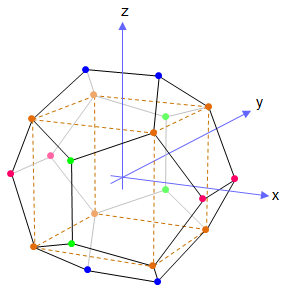
\includegraphics{Dodecahedron_vertices.png}
    \begin{solution} 我们先观察正十二面体,易发现旋转可以将一个面可以变到任意一个面,将十二个面的集合表示为
        $$
        X = \{1,2,3,\cdots ,12\}
        $$
        则$|O_1| = 12$,现在考虑$S_1$的大小,是这个面不动的置换包括以垂直于这个面中心的轴旋转的置换,有5个。
        所以$|G|=|O_1||S_1| = 60$。
    \end{solution}
\end{problem}

\end{document}